% ============================================================
% BÁO CÁO THỰC TẬP - VNPT AI
% Đề tài: Xây dựng Pipeline ETL và Tối ưu hóa Cơ sở dữ liệu
%         cho Hệ thống Chat thời gian thực
% ============================================================
\documentclass[12pt,a4paper]{article}

% === PACKAGES ===
\usepackage[utf8]{inputenc}
\usepackage[vietnamese]{babel}
\usepackage{graphicx}
\usepackage{geometry}
\usepackage{hyperref}
\usepackage{listings}
\usepackage{xcolor}
\usepackage{booktabs}
\usepackage{float}
\usepackage{caption}
\usepackage{subcaption}
\usepackage{fancyhdr}
\usepackage{titlesec}
\usepackage{enumitem}
\usepackage{amsmath}

% === PAGE SETUP ===
\geometry{left=2.5cm, right=2cm, top=2.5cm, bottom=2.5cm}

% === HEADER/FOOTER ===
\pagestyle{fancy}
\fancyhf{}
\fancyhead[L]{\small Báo Cáo Thực Tập - VNPT AI}
\fancyhead[R]{\small Nguyễn Phúc Bách}
\fancyfoot[C]{\thepage}
\renewcommand{\headrulewidth}{0.4pt}

% === CODE LISTING STYLE ===
\definecolor{codebg}{HTML}{F8F8F8}
\definecolor{codegreen}{HTML}{2ECC71}
\definecolor{codegray}{HTML}{7F8C8D}
\definecolor{codepurple}{HTML}{9B59B6}
\definecolor{codeblue}{HTML}{3498DB}

\lstdefinestyle{pythonstyle}{
    backgroundcolor=\color{codebg},
    commentstyle=\color{codegray}\itshape,
    keywordstyle=\color{codeblue}\bfseries,
    stringstyle=\color{codegreen},
    basicstyle=\ttfamily\small,
    breaklines=true,
    frame=single,
    rulecolor=\color{codegray!30},
    numbers=left,
    numberstyle=\tiny\color{codegray},
    numbersep=8pt,
    tabsize=4,
    showstringspaces=false
}

\lstdefinestyle{sqlstyle}{
    backgroundcolor=\color{codebg},
    commentstyle=\color{codegray}\itshape,
    keywordstyle=\color{codepurple}\bfseries,
    stringstyle=\color{codegreen},
    basicstyle=\ttfamily\small,
    breaklines=true,
    frame=single,
    rulecolor=\color{codegray!30},
    numbers=left,
    numberstyle=\tiny\color{codegray},
    numbersep=8pt,
    tabsize=4,
    showstringspaces=false,
    morekeywords={CREATE, KEYSPACE, TABLE, PRIMARY, KEY, WITH, AND, SELECT, FROM, WHERE, LIMIT, INSERT, INTO, VALUES}
}

\lstset{style=pythonstyle}

% === TITLE FORMATTING ===
\titleformat{\section}{\Large\bfseries}{\thesection.}{0.5em}{}
\titleformat{\subsection}{\large\bfseries}{\thesubsection.}{0.5em}{}

% === GRAPHICS PATH ===
\graphicspath{{images/}}

% ============================================================
\begin{document}

% === TRANG BÌA ===
\begin{titlepage}
    \centering
    \vspace*{1cm}

    {\Large\textbf{TỔNG CÔNG TY TRUYỀN THÔNG (VNPT-MEDIA)}}\\[0.3cm]
    {\large Trung tâm Nghiên cứu và Phát triển Trí tuệ Nhân tạo}\\[2cm]

    \rule{\textwidth}{1pt}\\[0.5cm]
    {\LARGE\textbf{BÁO CÁO THỰC TẬP}}\\[0.3cm]
    {\Large Xây dựng Pipeline ETL và Tối ưu hóa\\
    Cơ sở dữ liệu cho Hệ thống Chat thời gian thực}\\[0.5cm]
    \rule{\textwidth}{1pt}\\[2cm]

    \begin{flushleft}
        \large
        \textbf{Thực tập sinh:} Nguyễn Phúc Bách \\[0.3cm]
        \textbf{Đơn vị:} VNPT-AI \\[0.3cm]
        \textbf{Thời gian:} Tháng 07/2026 -- Tháng 08/2026 \\[0.3cm]
        \textbf{Công nghệ chính:} Apache Cassandra, ScyllaDB, Apache Spark (PySpark), Docker
    \end{flushleft}

    \vfill
    {\large Hà Nội, Tháng 08/2026}
\end{titlepage}

% === MỤC LỤC ===
\tableofcontents
\newpage

% ============================================================
% PHASE 0: THIẾT LẬP MÔI TRƯỜNG
% ============================================================
\section{Phase 0: Thiết lập Môi trường Phát triển}
\label{sec:phase0}

\subsection{Mục tiêu}
Thiết lập môi trường phát triển cục bộ (local development) bao gồm cơ sở dữ liệu nguồn (Cassandra), cơ sở dữ liệu đích (ScyllaDB), và công cụ xử lý dữ liệu (PySpark thông qua Jupyter Notebook). Toàn bộ hệ thống được đóng gói bằng Docker Compose.

\subsection{Kiến trúc Hạ tầng}

\begin{figure}[H]
    \centering
    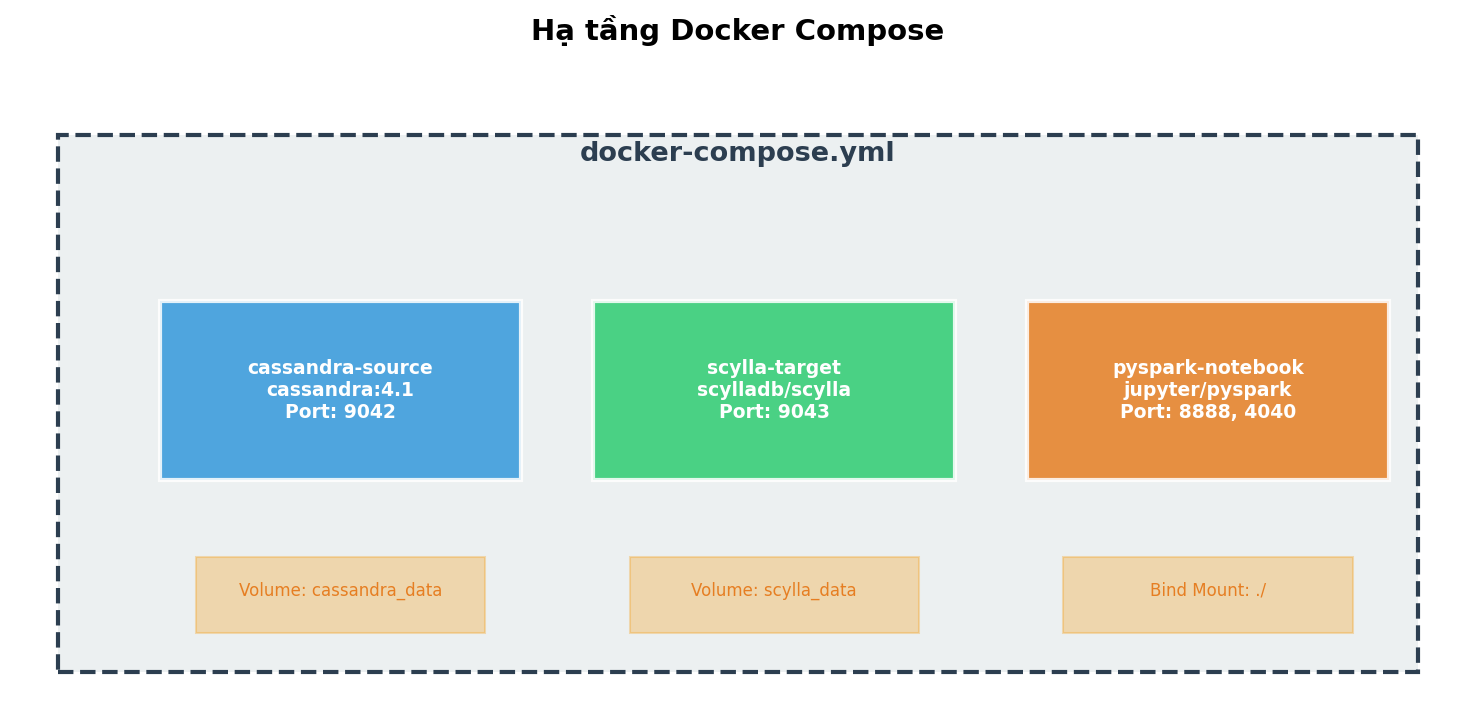
\includegraphics[width=0.85\textwidth]{docker_infrastructure.png}
    \caption{Sơ đồ kiến trúc hạ tầng Docker Compose gồm 3 container và các volume tương ứng.}
    \label{fig:docker}
\end{figure}

Hệ thống được triển khai gồm 3 container:

\begin{table}[H]
\centering
\caption{Thông số cấu hình các container trong \texttt{docker-compose.yml}}
\label{tab:containers}
\begin{tabular}{llll}
\toprule
\textbf{Service} & \textbf{Image} & \textbf{Port} & \textbf{Vai trò} \\
\midrule
cassandra-source & cassandra:4.1 & 9042 & Cơ sở dữ liệu nguồn \\
scylla-target & scylladb/scylla:latest & 9043 & Cơ sở dữ liệu đích \\
pyspark-notebook & jupyter/pyspark-notebook & 8888 & Môi trường phân tích \\
\bottomrule
\end{tabular}
\end{table}

\subsection{Dữ liệu Giả lập (Mock Data)}

Script \texttt{generate\_mock\_data.py} sinh khoảng 20.000 bản ghi tin nhắn chat với các đặc điểm:
\begin{itemize}[noitemsep]
    \item Nội dung tin nhắn bằng tiếng Việt, phản ánh ngữ cảnh chăm sóc khách hàng thực tế.
    \item Phân phối thiết bị theo trọng số: iOS (60\%), Android (30\%), Web (5\%), Desktop (5\%).
    \item Phân phối thời gian giả lập hành vi người dùng (giảm 2h--4h sáng, tăng 19h--21h tối).
    \item \texttt{room\_999} chứa 80\% tổng lượng dữ liệu nhằm mô phỏng tình trạng Hot Partition.
\end{itemize}

\begin{figure}[H]
    \centering
    \begin{subfigure}[b]{0.48\textwidth}
        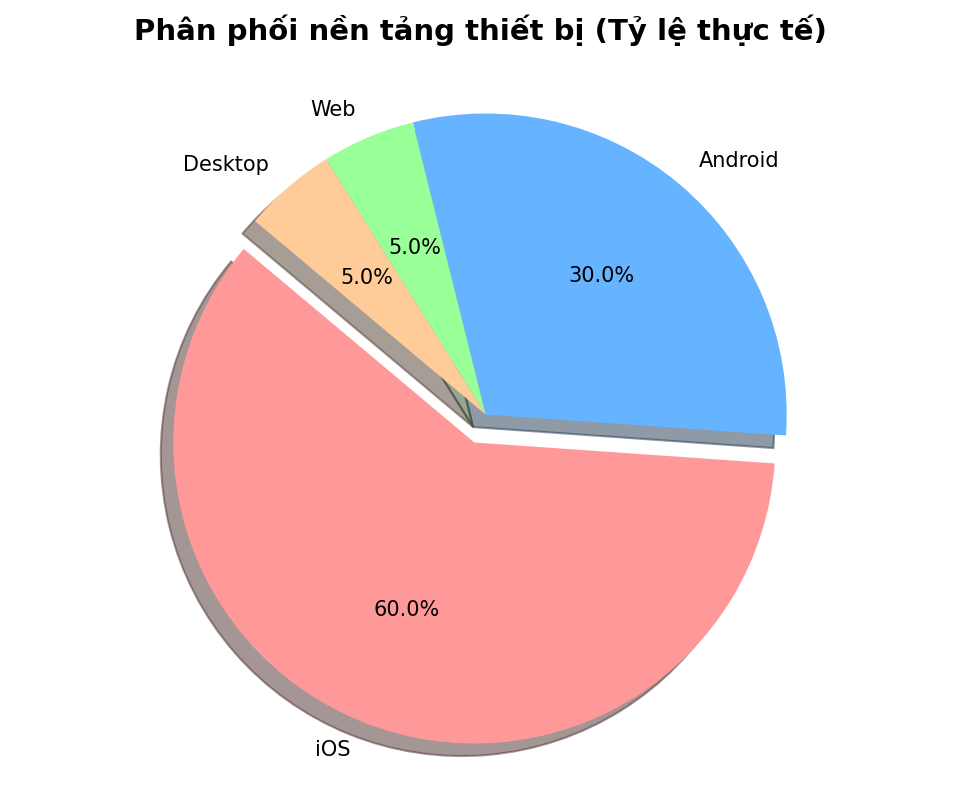
\includegraphics[width=\textwidth]{device_distribution.png}
        \caption{Phân phối nền tảng thiết bị.}
        \label{fig:device}
    \end{subfigure}
    \hfill
    \begin{subfigure}[b]{0.48\textwidth}
        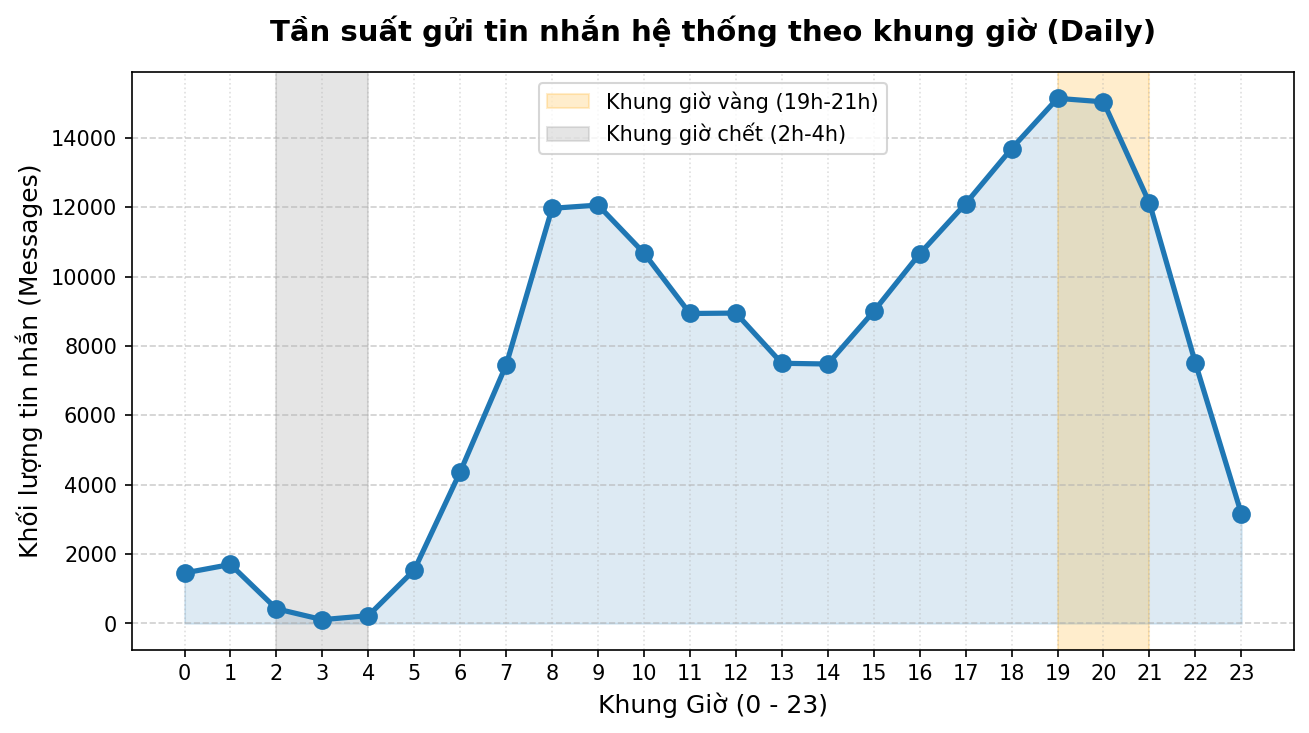
\includegraphics[width=\textwidth]{time_distribution.png}
        \caption{Phân phối tần suất tin nhắn theo giờ.}
        \label{fig:time}
    \end{subfigure}
    \caption{Các biểu đồ phân phối dữ liệu giả lập, phản ánh hành vi sử dụng thực tế.}
    \label{fig:mock_data}
\end{figure}

% ============================================================
% PHASE 1: PHÂN TÍCH DỮ LIỆU
% ============================================================
\newpage
\section{Phase 1: Phân tích Dữ liệu Khám phá (EDA)}
\label{sec:phase1}

\subsection{Mục tiêu}
Thực hiện Exploratory Data Analysis trên dữ liệu nguồn (Cassandra) để xác định các vấn đề về hiệu năng và phân phối dữ liệu.

\subsection{Kết quả Phân tích}

\begin{figure}[H]
    \centering
    \begin{subfigure}[b]{0.48\textwidth}
        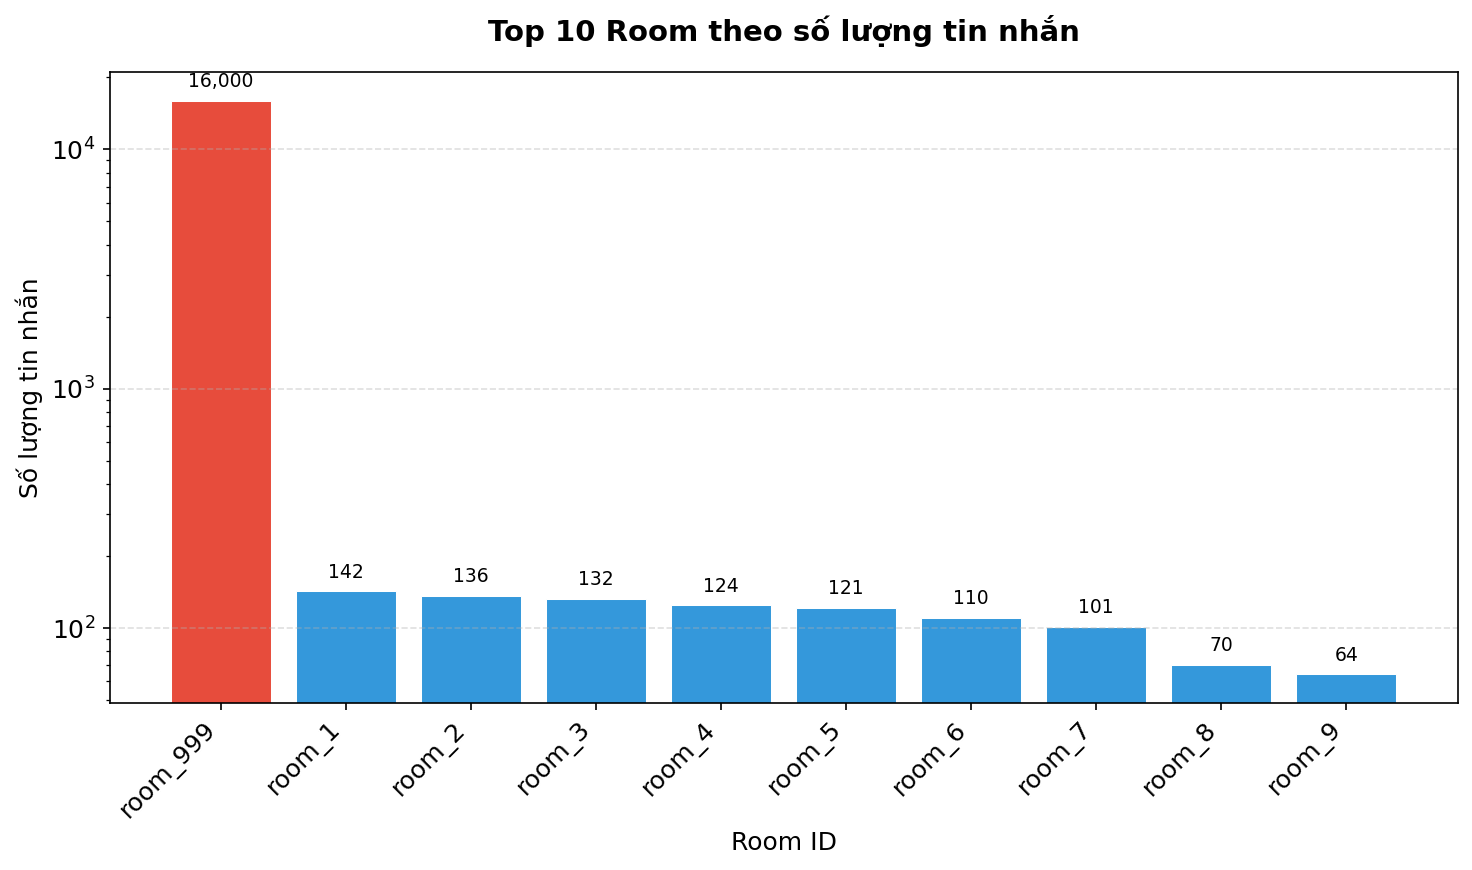
\includegraphics[width=\textwidth]{room_distribution.png}
        \caption{Phân phối số lượng tin nhắn theo Room (log scale). \texttt{room\_999} chiếm 80\% tổng dữ liệu.}
        \label{fig:room_dist}
    \end{subfigure}
    \hfill
    \begin{subfigure}[b]{0.48\textwidth}
        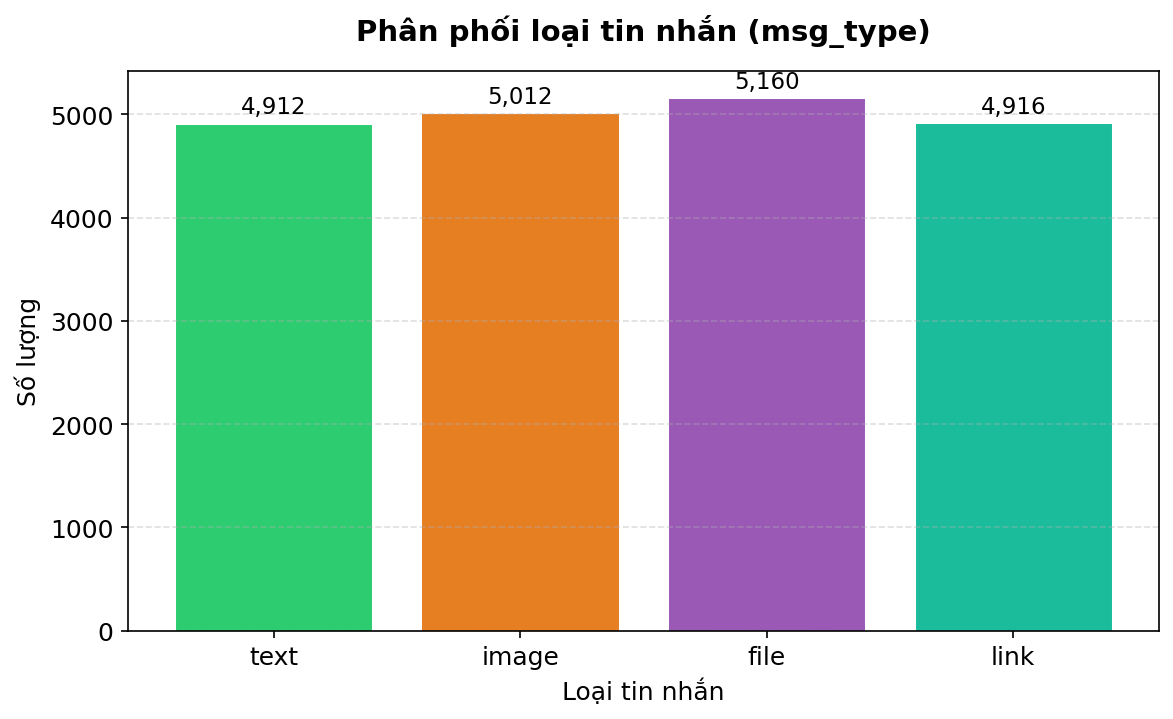
\includegraphics[width=\textwidth]{msg_type_distribution.png}
        \caption{Phân phối loại tin nhắn (text, image, file, link).}
        \label{fig:msg_type}
    \end{subfigure}
    \caption{Kết quả EDA từ tập dữ liệu nguồn trên Cassandra.}
    \label{fig:eda}
\end{figure}

\textbf{Phát hiện chính:}
\begin{itemize}[noitemsep]
    \item \texttt{room\_999} chứa khoảng 16.000 tin nhắn trên tổng 20.000, tạo hiện tượng Hot Partition.
    \item 20 phòng chat còn lại phân bổ đồng đều, trung bình 50--150 tin nhắn mỗi phòng.
    \item Phân phối Hot Partition này là cơ sở cho quyết định thiết kế Time-bucketing ở Phase 2.
\end{itemize}

% ============================================================
% PHASE 2: THIẾT KẾ SCYLLADB
% ============================================================
\newpage
\section{Phase 2: Thiết kế Kiến trúc ScyllaDB}
\label{sec:phase2}

\subsection{Mục tiêu}
Thiết kế lại cấu trúc cơ sở dữ liệu (schema) trên ScyllaDB để khắc phục vấn đề Hot Partition và tối ưu hóa hiệu năng truy vấn.

\subsection{So sánh Schema Cũ và Mới}

\begin{figure}[H]
    \centering
    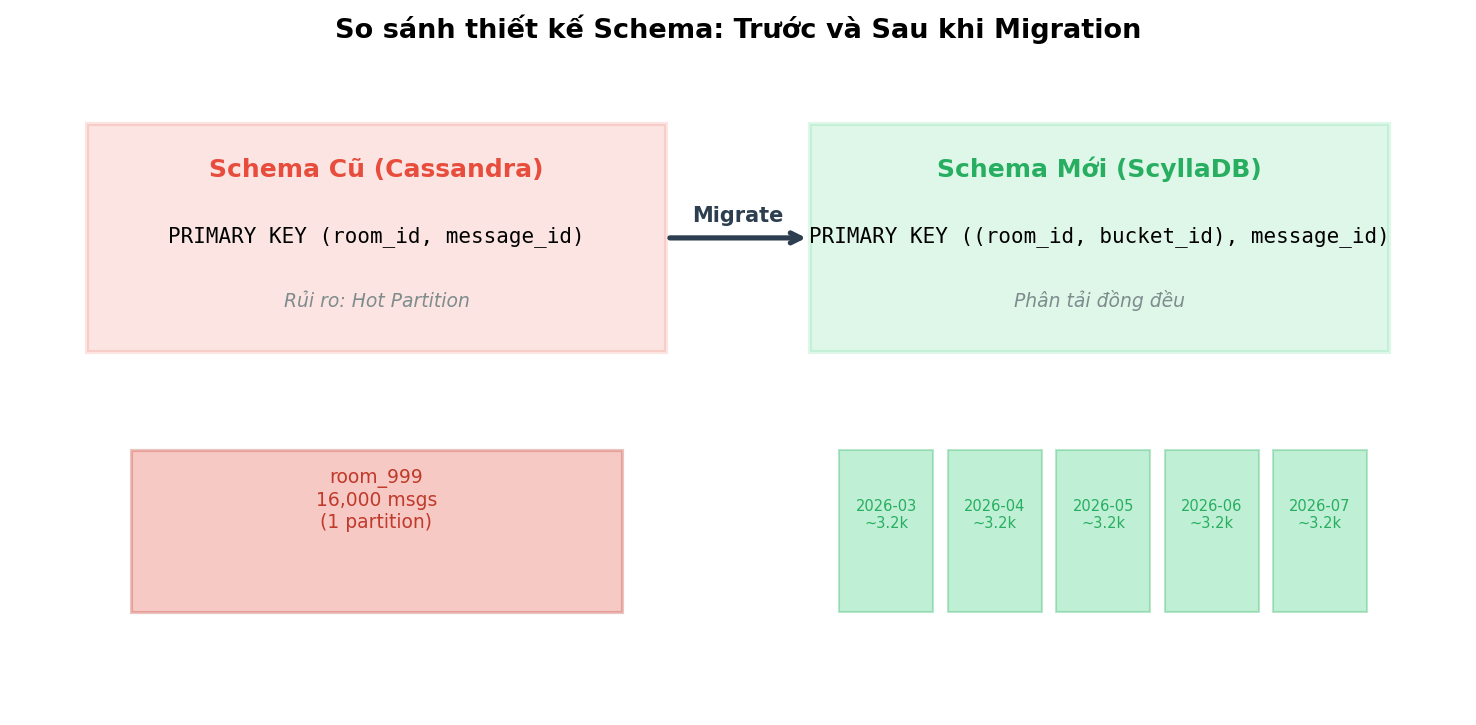
\includegraphics[width=0.9\textwidth]{schema_comparison.png}
    \caption{So sánh thiết kế schema trước và sau khi migration. Dữ liệu \texttt{room\_999} được phân tán từ 1 partition thành 5 partitions nhỏ theo tháng.}
    \label{fig:schema}
\end{figure}

\begin{table}[H]
\centering
\caption{So sánh cấu trúc Primary Key giữa hai phiên bản schema.}
\label{tab:schema}
\begin{tabular}{lll}
\toprule
 & \textbf{Schema cũ (Cassandra)} & \textbf{Schema mới (ScyllaDB)} \\
\midrule
Partition Key & \texttt{room\_id} & \texttt{(room\_id, bucket\_id)} \\
Clustering Key & \texttt{message\_id DESC} & \texttt{message\_id DESC} \\
Rủi ro & Hot Partition & Không \\
\bottomrule
\end{tabular}
\end{table}

\subsection{Quản lý Vòng đời Dữ liệu}

\begin{itemize}[noitemsep]
    \item \textbf{TimeWindowCompactionStrategy (TWCS):} Nhóm SSTable theo khung thời gian 1 ngày, tối ưu hóa quá trình xóa dữ liệu cũ.
    \item \textbf{TTL:} \texttt{default\_time\_to\_live = 2592000} (30 ngày). Tỷ lệ TTL/window duy trì $< 50$ theo giới hạn của ScyllaDB.
    \item \textbf{Tombstone:} Bản ghi hết hạn giữ tombstone trong \texttt{gc\_grace\_seconds} (10 ngày) để hoàn tất sync giữa các replica.
\end{itemize}

\subsection{Mẫu Truy vấn cho Backend}

\begin{lstlisting}[style=sqlstyle, caption={Truy xuất 50 tin nhắn mới nhất của một phòng chat.}]
SELECT * FROM chat_system_target.chat_table_bucketed
WHERE room_id = 'room_1' AND bucket_id = '2026-07'
LIMIT 50;
\end{lstlisting}

\begin{lstlisting}[style=sqlstyle, caption={Truy vấn phân trang (pagination) lịch sử tin nhắn.}]
SELECT * FROM chat_system_target.chat_table_bucketed
WHERE room_id = 'room_1' AND bucket_id = '2026-07'
  AND message_id < 6ff1b35a-8405-11f1-8e64-af4db1424c6c
LIMIT 50;
\end{lstlisting}

% ============================================================
% PHASE 3: PIPELINE ETL
% ============================================================
\newpage
\section{Phase 3: Pipeline ETL bằng PySpark}
\label{sec:phase3}

\subsection{Mục tiêu}
Xây dựng pipeline ETL để di dời dữ liệu từ Cassandra sang ScyllaDB, kèm theo tối ưu hóa hiệu năng và hệ thống lưu trữ lạnh (Cold Archiver).

\subsection{Kiến trúc Pipeline}

\begin{figure}[H]
    \centering
    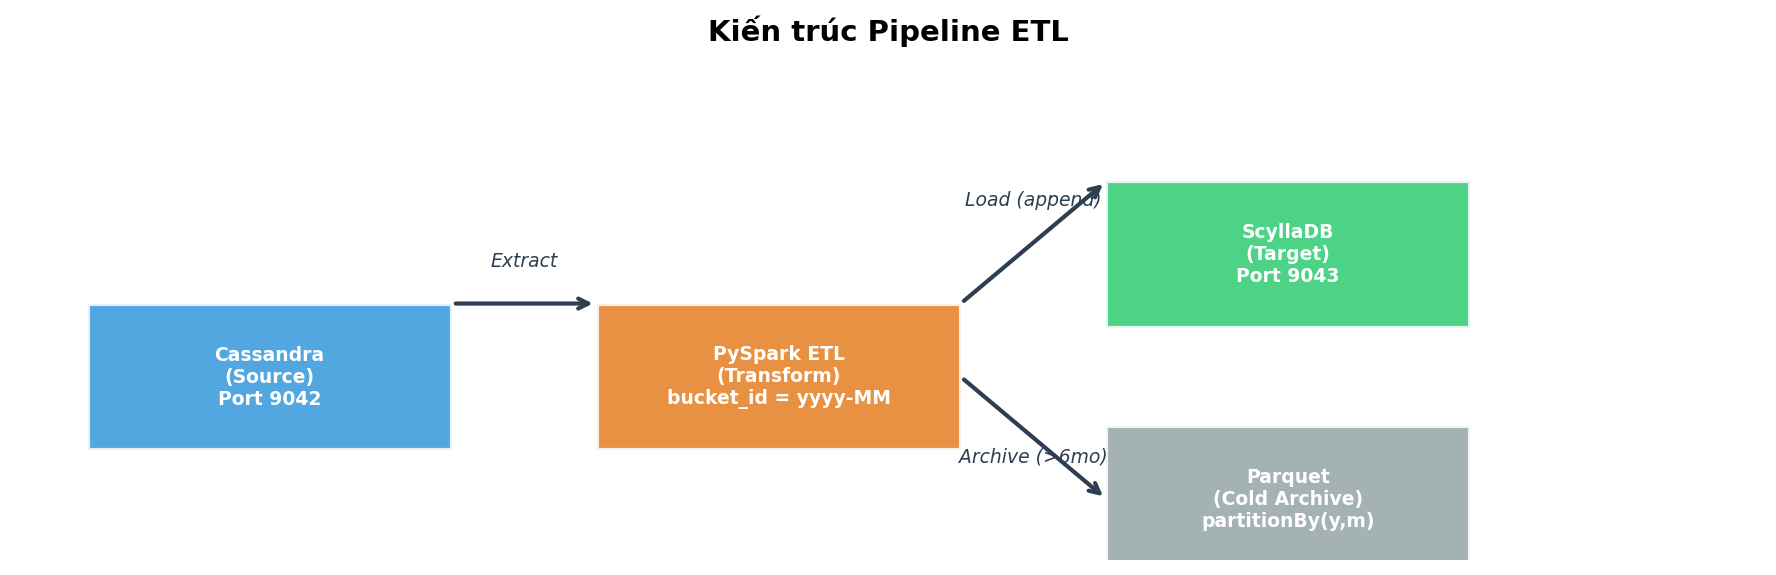
\includegraphics[width=0.9\textwidth]{etl_architecture.png}
    \caption{Sơ đồ kiến trúc Pipeline ETL: Extract từ Cassandra, Transform (thêm \texttt{bucket\_id}), Load vào ScyllaDB hoặc xuất Parquet.}
    \label{fig:etl_arch}
\end{figure}

\subsection{Triển khai ETL (Tuần 5)}

\textbf{Cấu hình môi trường:} Lỗi \texttt{ClassNotFound} khi kết nối Cassandra được xử lý bằng cách khai báo biến môi trường \texttt{PYSPARK\_SUBMIT\_ARGS}, cho phép Spark tự động tải gói dependency (\texttt{.jar}).

\begin{figure}[H]
    \centering
    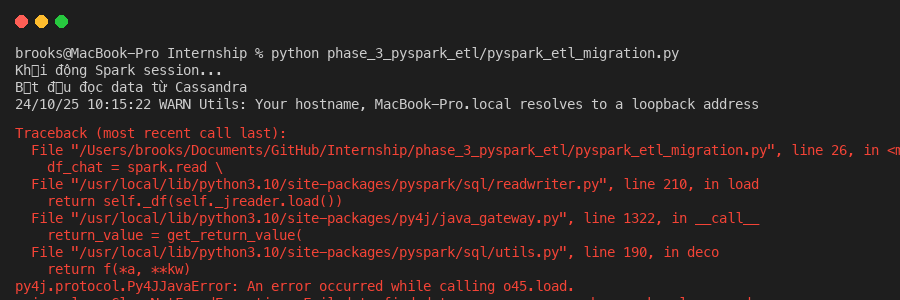
\includegraphics[width=0.7\textwidth]{cassandra_class_not_found.png}
    \caption{Thông báo lỗi thiếu thư viện dependency trong quá trình thực thi.}
    \label{fig:error}
\end{figure}

\textbf{Xử lý Hot Partition:} Bước Transform bổ sung trường \texttt{bucket\_id} (định dạng \texttt{yyyy-MM}) bằng hàm \texttt{date\_format} của PySpark.

\begin{lstlisting}[language=Python, caption={Logic Transform: thêm trường \texttt{bucket\_id} cho Time-bucketing.}]
df_transformed = df_source.withColumn(
    "bucket_id", date_format(col("timestamp"), "yyyy-MM")
)
\end{lstlisting}

\textbf{Load:} Pipeline sử dụng \texttt{.mode("append")} để ghi dữ liệu vào ScyllaDB, đảm bảo không ghi đè bản ghi hiện có.

\subsection{Tối ưu hóa Hiệu năng I/O (Tuần 6)}

\begin{figure}[H]
    \centering
    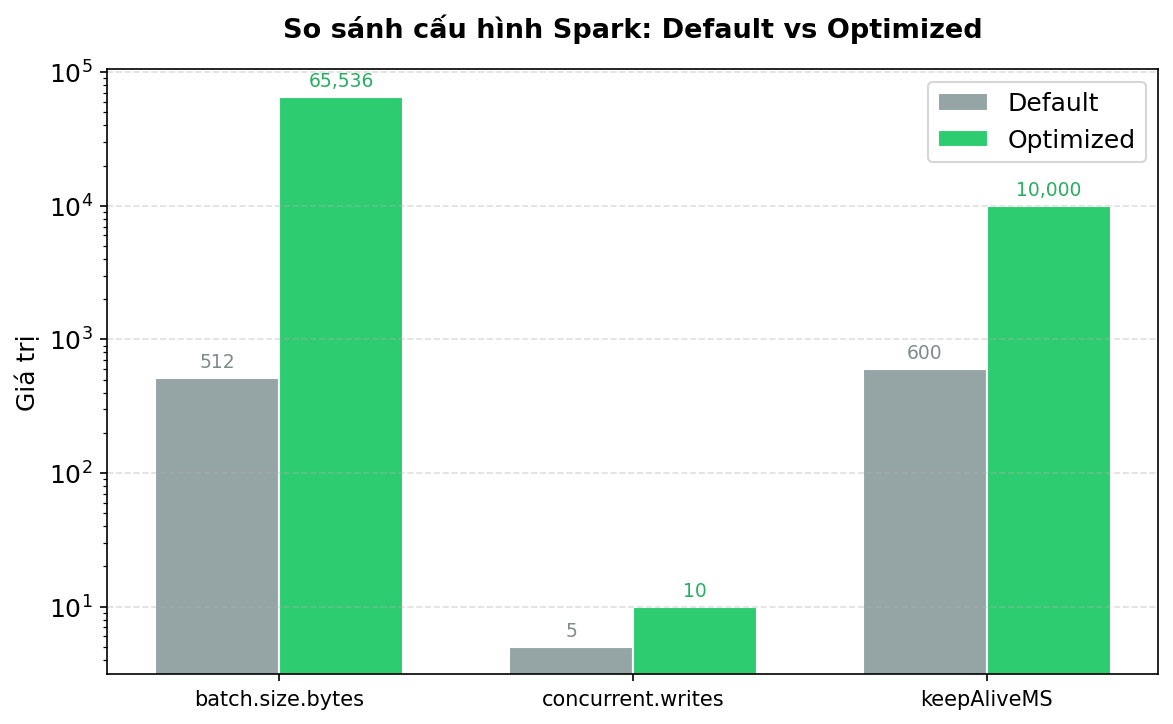
\includegraphics[width=0.7\textwidth]{spark_optimization.png}
    \caption{So sánh giá trị cấu hình Spark giữa chế độ Default và Optimized (log scale).}
    \label{fig:spark_opt}
\end{figure}

\begin{table}[H]
\centering
\caption{Bảng cấu hình Spark Cassandra Connector cho chế độ Optimized.}
\label{tab:spark_config}
\begin{tabular}{lrrl}
\toprule
\textbf{Tham số} & \textbf{Default} & \textbf{Optimized} & \textbf{Mục đích} \\
\midrule
\texttt{batch.size.bytes} & 512 & 65,536 & Gom batch, giảm overhead mạng \\
\texttt{concurrent.writes} & 5 & 10 & Tăng luồng ghi song song \\
\texttt{keepAliveMS} & 600 & 10,000 & Tái sử dụng connection pool \\
\bottomrule
\end{tabular}
\end{table}

\subsection{Cold Archiver (Tuần 7)}

Script \texttt{cold\_archiver.py} di chuyển dữ liệu cũ (> 6 tháng) sang kho lưu trữ dài hạn:
\begin{itemize}[noitemsep]
    \item Lọc dữ liệu bằng module \texttt{datetime} chuẩn Python.
    \item Xuất ra định dạng \textbf{Parquet} với \texttt{partitionBy("year", "month")}.
    \item Thiết kế đọc dữ liệu 1-Pass, loại bỏ \texttt{.count()} để tránh quá tải bộ nhớ.
\end{itemize}

% ============================================================
% TỔNG KẾT
% ============================================================
\newpage
\section{Tổng kết}

\subsection{Kết quả đạt được}

\begin{table}[H]
\centering
\caption{Tổng hợp kết quả theo từng Phase.}
\label{tab:summary}
\begin{tabular}{lll}
\toprule
\textbf{Phase} & \textbf{Nội dung} & \textbf{Trạng thái} \\
\midrule
Phase 0 & Thiết lập Docker Compose, sinh Mock Data & Hoàn thành \\
Phase 1 & Phân tích EDA, phát hiện Hot Partition & Hoàn thành \\
Phase 2 & Thiết kế schema ScyllaDB, Time-bucketing & Hoàn thành \\
Phase 3 & Pipeline ETL, Tối ưu I/O, Cold Archiver & Hoàn thành \\
\bottomrule
\end{tabular}
\end{table}

\subsection{Công nghệ sử dụng}

\begin{table}[H]
\centering
\caption{Danh sách công nghệ và thư viện chính.}
\label{tab:tech}
\begin{tabular}{ll}
\toprule
\textbf{Công nghệ} & \textbf{Phiên bản / Vai trò} \\
\midrule
Apache Cassandra & 4.1 (Cơ sở dữ liệu nguồn) \\
ScyllaDB & latest (Cơ sở dữ liệu đích) \\
Apache Spark (PySpark) & 3.4.x (Xử lý ETL) \\
Docker Compose & 3.8 (Đóng gói hạ tầng) \\
Python & 3.x (Scripting, Mock Data) \\
cassandra-driver & Kết nối Python $\leftrightarrow$ Cassandra/ScyllaDB \\
Matplotlib & Trực quan hóa dữ liệu \\
\bottomrule
\end{tabular}
\end{table}

\subsection{Hướng phát triển tiếp theo}

\begin{enumerate}[noitemsep]
    \item \textbf{Phase 4 -- Phân tích NLP:} Tiền xử lý văn bản tiếng Việt, phân tích cảm xúc (Sentiment Analysis) trên tập dữ liệu tin nhắn chat.
    \item \textbf{Trực quan hóa:} Xây dựng Dashboard tổng hợp các chỉ số hệ thống (WordCloud, biểu đồ giờ cao điểm).
    \item \textbf{Giám sát Production:} Tích hợp hệ thống monitoring (Prometheus/Grafana) cho cụm ScyllaDB.
\end{enumerate}

\end{document}
